% !TeX root = main.tex
\chapter{Introduction}\label{chp:intro}

Want to improve interface for professionally working with audio content

Semantic audio analysis can extract useful information, but how can this best be used?

Tasks are creative, so can't easily be automated

Humans and machines working to their strengths

\section{Background and motivation}\label{sec:intro-motivation}
Ever since the first digital audio workstations were introduced in the early
1990s, the audio waveform has been the primary method of navigating audio
content. The waveform works well for finding amplitude-related events such as
silences and peaks, but is very poor at conveying much more about the sound of
the content. Additionally, the waveform doesn't scale well as demonstrated by
the `Soundcloud sausage' (see Figure~\ref{fig:soundcloud}), where even at
reasonable zoom levels, no useful information is presented.  A popular
alternative to the waveform is the spectrogram, which displays detailed
information about the frequency content. However, these can be very difficult
to interpret and require training and practice to be of use.

\begin{figure}[ht]
  \centering
  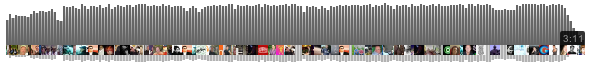
\includegraphics[width=0.6\textwidth]{figs/soundcloud.png}
  \caption{An example of a waveform visualization on the online music sharing
    service Soundcloud}
  \label{fig:soundcloud}
\end{figure}

\section{Research questions and scope}\label{sec:intro-questions}
This projects aims to develop better visualization for helping radio producers
navigate audio content by initially targeting a number of common tasks. Audio
features will be identified or developed which are able to capture the
information required for the task. Methods of mapping these features to an
image will be created so that the information is presented in a perceptible way
which requires little or no training. 

\section{Thesis structure}\label{sec:intro/structure}

\paragraph{Chapter \ref{chp:background}} reviews existing work and literature
from three areas that will feed into the project -- feature extraction,
visualization and cross-modal links.

\paragraph{Chapter \ref{chp:colourised}} details the process and results of an
initial online study which looked at how the waveform performs in a common
production tasks, and whether it can be improved.

\paragraph{Chapter \ref{chp:ethno}} provides a comprehensive overview of
the radio production process at the BBC, which will help put this research into
context.

\paragraph{Chapter \ref{chp:screen}} investigates how a screen-based semantic audio editing interface affects the
production process.

\paragraph{Chapter \ref{chp:paper}} investigates how a paper-based semantic audio editing interface compares to
the screen-based approach and normal paper.

\paragraph{Chapter \ref{chp:conclusions}} concludes the thesis and considers the prospects for future research.

\section{Contributions}\label{sec:intro-contributions}

The principal contributions of this thesis are:
\begin{itemize}
  \item Chapter~\ref{chp:colourised}: 
  \item Chapter~\ref{chp:ethno}: 
  \item Chapter~\ref{chp:screen}: 
  \item Chapter~\ref{chp:paper}: a novel system for editing speech-based audio using digital pens on printed transcripts
  \item Appendix~\ref{sec:discourse}: an open-source semantic audio editing system
  \item Appendix~\ref{sec:vampeyer}: an open-source audio visualisation plugin framework
  \item Appendix~\ref{sec:beatmap}: an open-source library for rendering tiled audio visualisation in web browsers
\end{itemize}

%In addition, this work has produced the following technological developments:
%
%\begin{itemize}
%  \item `Discourse' -- a screen-based semantic audio editing system, available as open source
%    software\footnote{\url{https://github.com/bbc/discourse}}. See Section~\ref{sec:discourse}.
%  \item A digital pen system for editing audio using printed transcripts.
%  \item `Vampeyer' -- an audio visualisation plugin framework, available as open source
%    software\footnote{\url{https://github.com/bbc/vampeyer}}. See Section~\ref{sec:vampeyer}.
%  \item `Beatmap' -- a Javascript user interface element for audio visualisation based on tiled bitmaps, available as
%    open source software\footnote{\url{https://github.com/bbc/beatmap}}. See Section~\ref{sec:beatmap}.
%\end{itemize}

\section{Associated publications}\label{sec:intro-publications}

Portions of the work detailed in this thesis have been presented in the following publications:

\begin{itemize}
  \item Chapter~\ref{chp:ethno}: The results of this work were published and presented at the 138th Audio Engineering Society Conference in
    Warsaw, Poland \citep{Baume2015}
\end{itemize}
